\documentclass[final]{beamer}

\usepackage[size=a0,orientation=portrait,scale=1.22]{beamerposter}
\usepackage{amsmath,amssymb}
\usepackage{booktabs}
\usepackage{graphicx}
\usepackage{ragged2e}
\usepackage{array}
\usepackage{xcolor}
\usepackage{hyperref}

\graphicspath{{./}{../results/figures/standard/}{../results/figures_theta/}}

\definecolor{posterblue}{RGB}{43,66,143}
\definecolor{postergreen}{RGB}{30,132,91}
\definecolor{posterred}{RGB}{190,59,48}
\definecolor{sectiongray}{RGB}{235,239,246}
\definecolor{ink}{RGB}{20,25,34}
\definecolor{muted}{RGB}{85,93,110}

\usetheme{default}
\usefonttheme{serif}
\setbeamertemplate{navigation symbols}{}
\setbeamertemplate{caption}[numbered]
\setbeamersize{text margin left=0pt,text margin right=0pt}
\setbeamercolor{normal text}{fg=ink,bg=white}
\setbeamercolor{section title}{fg=posterblue,bg=sectiongray}

\newlength{\postercontentwidth}
\setlength{\postercontentwidth}{0.955\paperwidth}

\newcommand{\sechead}[2]{%
  \vspace{0.34cm}
  \begin{beamercolorbox}[wd=\linewidth,sep=0.20cm,leftskip=0.24cm]{section title}
    {\Large\bfseries #1. #2}
  \end{beamercolorbox}
  \vspace{0.20cm}
}

\newcommand{\bluebox}[1]{%
  \begingroup
  \setlength{\fboxsep}{0.30cm}
  \setlength{\fboxrule}{1.1pt}
  \noindent\fcolorbox{posterblue}{white}{%
    \begin{minipage}{0.94\linewidth}
    \color{ink}#1
    \end{minipage}}%
  \endgroup
}

\newcommand{\statbox}[2]{%
  \begin{minipage}[t]{0.31\linewidth}
    \centering
    {\large\bfseries\color{postergreen}#1}\\[-0.04cm]
    {\tiny\color{muted}#2}
  \end{minipage}
}

\newcommand{\tightitems}{\setlength\itemsep{0.12em}\setlength\parskip{0pt}}

\title{Opportunistic Target Selection}
\subtitle{Early Directional Commitment for Query-Efficient Black-Box Adversarial Attacks}
\author{Florent Tariolle and Florian Yger}
\institute{INSA Rouen Normandy; LITIS}

\begin{document}
\begin{frame}[t]
\normalsize
\setlength{\parindent}{0pt}
\setlength{\parskip}{0.14cm}
\justifying

% Header.
\noindent\makebox[\paperwidth][c]{%
\begin{minipage}{\postercontentwidth}
\vspace{0.55cm}
\begin{minipage}[c]{0.20\linewidth}
  \centering
  
\includegraphics[width=11.2cm]{school_logo.png}\\[0.28cm]
  
\includegraphics[width=7.2cm]{logo_LITIS_cropped.png}
\end{minipage}
\hfill
\begin{minipage}[c]{0.58\linewidth}
  \centering
  {\Huge\bfseries\color{posterblue}\inserttitle\par}
  \vspace{0.20cm}
  {\LARGE\bfseries\color{posterblue}\insertsubtitle\par}
  \vspace{0.26cm}
  {\Large Florent Tariolle\textsuperscript{1} \quad Florian Yger\textsuperscript{1,2}\par}
  {\large \textsuperscript{1}INSA Rouen Normandy \quad \textsuperscript{2}LITIS \quad -- \quad CAp 2026 A Poster\par}
\end{minipage}
\hfill
\begin{minipage}[c]{0.16\linewidth}
  \hfill
  \begin{minipage}{7.6cm}
    \centering
    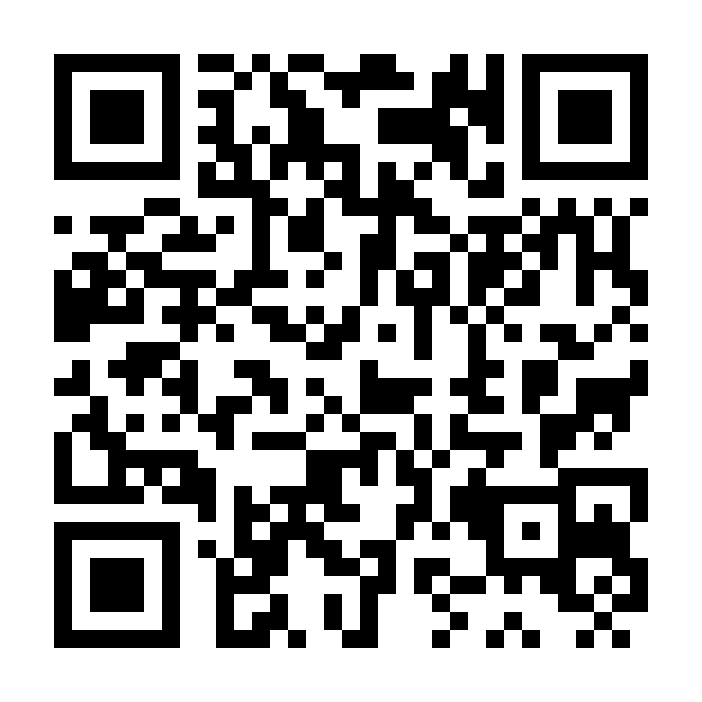
\includegraphics[width=\linewidth]{arxiv_qr.png}\\[-0.05cm]
    {\small\href{https://arxiv.org/abs/2605.25663}{arXiv:2605.25663}}
  \end{minipage}
\end{minipage}
\vspace{0.38cm}
\end{minipage}}

\vspace{0.10cm}
{\color{posterblue}\rule{\paperwidth}{1.4pt}}

\vspace{0.28cm}
\noindent\makebox[\paperwidth][c]{%
\begin{minipage}{\postercontentwidth}
\noindent%
\begin{minipage}[t]{0.485\linewidth}

\sechead{1}{Setup \& Motivation}
Score-based black-box attacks observe the model probabilities but not gradients. Standard untargeted attacks reduce only the true-class confidence:
\[
\mathcal{L}_{\mathrm{untarg}}(x',y)=P(y\mid x')\quad\text{or}\quad \log P(y\mid x').
\]
This objective frees probability mass without deciding which non-true class should receive it. The attack may therefore drift across several class basins before a misclassification is reached.

\bluebox{\textbf{Goal.} Use the attack trajectory itself to choose a viable adversarial target, then commit early enough to avoid wasting queries on class drift.}

\textbf{Why this gap exists.} Targeted attacks remove drift but require a target before the attack starts. Margin losses track a competitor dynamically, but many score-based attacks are implemented with probability or CE losses. OTS is a wrapper for exactly that case.

\sechead{2}{Method: Opportunistic Target Selection}
OTS leaves the proposal mechanism unchanged. It modifies only the loss schedule after a short untargeted prefix.

\bluebox{%
\textbf{Algorithm.}
\begin{enumerate}
  \tightitems
  \item Run the original untargeted attack for $T$ iterations.
  \item Lock onto the leading non-true class
  \[
  t=\arg\max_{k\neq y}P(k\mid x'_T).
  \]
  \item Continue the same attack, but maximize the target confidence $P(t\mid x')$.
  \item Stop when the classifier prediction is no longer $y$.
\end{enumerate}}

The lock is deliberately irreversible. Releasing it would reintroduce the exploration overhead that OTS is meant to remove. Across fixed switches $T\in\{5,\ldots,500\}$, performance is statistically indistinguishable, so the useful class ranking stabilizes very early.

\sechead{3}{Experimental Protocol}
\begin{center}
\begin{tabular}{@{}>{\bfseries}p{0.23\linewidth}p{0.68\linewidth}@{}}
\toprule
Models & AlexNet, ResNet-18, VGG-16, ResNet-50, ViT-B/16 \\
Attacks & SimBA, Square Attack with CE loss, Bandits \\
Modes & Untargeted baseline, targeted oracle, OTS \\
Budget & $\epsilon=8/255$ in $L_\infty$, 10K iterations \\
Scale & 100 ImageNet images per model, 4,500 standard-model runs \\
Metrics & Success rate and censored mean iterations \\
\bottomrule
\end{tabular}
\end{center}

\bluebox{\textbf{Oracle target.} The oracle is the class reached by a same-seed untargeted probe. It is a trajectory-specific ceiling, not a deployable method.}

\sechead{4}{When Should OTS Help?}
\begin{center}
\begin{tabular}{@{}p{0.21\linewidth}p{0.23\linewidth}p{0.42\linewidth}@{}}
\toprule
Attack & Direction source & Expected OTS effect \\
\midrule
SimBA & No target tracking & Large gain from early commitment \\
Square CE & CE suppresses $y$ only & Gain similar to a margin surrogate \\
Bandits & Gradient estimate & Small or negative gain \\
\bottomrule
\end{tabular}
\end{center}

The negative Bandits case is part of the result, not a failure of tuning: once an attack already estimates a useful direction, imposing a fixed target can interfere with that direction.

\sechead{5}{Mechanism}
\begin{center}
\includegraphics[height=20.0cm,keepaspectratio]{fig_theta.pdf}
\end{center}

After lock-in, OTS aligns perturbations with the oracle direction. On SimBA/ResNet-50, terminal cosine similarity rises from $0.174$ for untargeted perturbations to $0.865$ for OTS.

\textbf{Interpretation.} Once OTS fixes $t$, maximizing $P(t\mid x')$ approximates the competitor term of margin loss:
\[
\mathcal{L}_{\mathrm{margin}}=f_y(x')-\max_{k\neq y}f_k(x').
\]
OTS is therefore a lightweight margin-loss surrogate for attacks that do not already track a competitor.

\sechead{6}{Target-Rule Ablation}
\begin{center}
\begin{tabular}{@{}lcc@{}}
\toprule
Target rule & SimBA & Square CE \\
\midrule
Random non-true class & 14\% & 53\% \\
Clean-image argmax & 79\% & 96\% \\
Short exploration & 80\% & 99\% \\
\bottomrule
\end{tabular}
\end{center}

Random targets are catastrophic. Clean-image rankings are already strong for SimBA, while Square Attack benefits from a short exploration phase because random patches disturb the initial ranking.

\end{minipage}%
\hfill%
\begin{minipage}[t]{0.485\linewidth}

\sechead{7}{Main Results}
\begin{center}
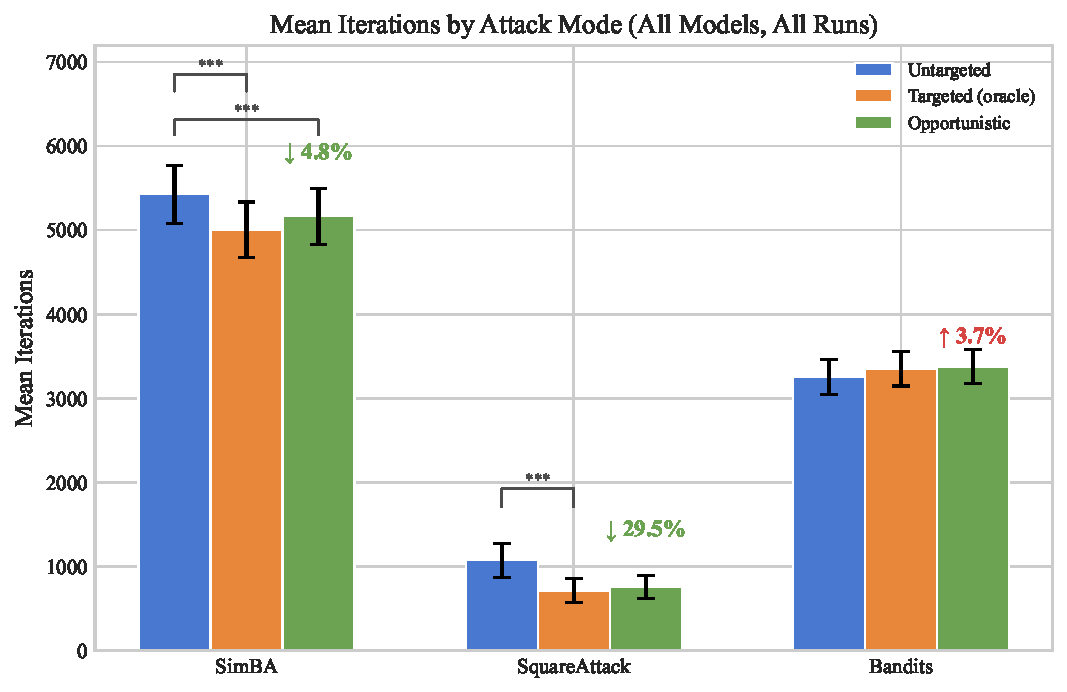
\includegraphics[height=20.0cm,keepaspectratio]{fig_headline_bars.pdf}
\end{center}

\vspace{-0.12cm}
\begin{center}
\begin{tabular}{@{}lccc@{}}
\toprule
Attack & Untargeted & OTS & Oracle \\
\midrule
SimBA & 67\% & \textbf{75\%} & 76\% \\
Square CE & 96\% & \textbf{99\%} & 99\% \\
Bandits & 37\% & 34\% & 35\% \\
\bottomrule
\end{tabular}
\end{center}

\begin{center}
\begin{tabular}{@{}>{\centering\arraybackslash}p{0.29\linewidth}>{\centering\arraybackslash}p{0.29\linewidth}>{\centering\arraybackslash}p{0.29\linewidth}@{}}
{\bfseries\color{postergreen}+27 pp} & {\bfseries\color{postergreen}43\%} & {\bfseries\color{postergreen}0} \\
{\scriptsize SimBA success on ResNet-50} & {\scriptsize relative iteration reduction} & {\scriptsize gradient access} \\
\end{tabular}
\end{center}

\bluebox{\textbf{Main finding.} OTS nearly matches the trajectory oracle for SimBA and Square Attack with CE loss, while Bandits gets worse because it already follows an estimated gradient direction.}

\sechead{8}{Lock-In Dynamics}
\begin{center}
\includegraphics[height=22.0cm,keepaspectratio,trim=0 45pt 436pt 24pt,clip]{fig_lockin.pdf}
\end{center}

In this ResNet-50 example, the faded untargeted trajectory suppresses the true class but then drifts. The vivid OTS trajectory locks onto class 988 and continues to increase that class until the attack succeeds.

\bluebox{\textbf{Practical point.} OTS does not need the exact oracle class in every run; it only needs a viable class that remains competitive after lock-in.}

\sechead{9}{Loss Interpretation}
\begin{center}
\begin{tabular}{@{}lcc@{}}
\toprule
Square Attack, ResNet-50 & Success & Mean iter. \\
\midrule
CE untargeted & 85.0\% & 2,601 \\
CE + OTS & 98.0\% & 1,791 \\
CE oracle & 99.0\% & 1,865 \\
Margin untargeted & 98.7\% & 1,453 \\
Margin + OTS & 98.7\% & 1,583 \\
\bottomrule
\end{tabular}
\end{center}

OTS repairs CE-style drift, but default margin loss already performs dynamic competitor tracking at every iteration. This explains why OTS is useful for CE variants and redundant for margin-based Square Attack.

\sechead{10}{Limits \& Future Work}
On adversarially trained ImageNet models, success rates are flat across untargeted, oracle, and OTS. The issue is not bad target selection; robust models remove the medium-difficulty regime where directional commitment pays off.

\bluebox{\textbf{Future work.} Test smaller-label regimes such as CIFAR-10, $L_2$ budgets, randomized defenses, and adaptive re-locking when the selected class drops in rank.}

\sechead{11}{Takeaways \& Links}
\bluebox{%
\textbf{Take-away.} OTS is a small loss-schedule change: explore briefly, lock onto the strongest non-true class, then optimize that class. It helps drift-prone score attacks and exposes when an attack already has enough directional information.}

{\footnotesize
[1] Guo et al., \textit{Simple Black-box Adversarial Attacks}, ICML 2019.\par
[2] Andriushchenko et al., \textit{Square Attack}, ECCV 2020.\par
[3] Ilyas et al., \textit{Prior Convictions}, ICLR 2019.\par
\vspace{0.08cm}
\textbf{Paper:} \href{https://arxiv.org/abs/2605.25663}{arxiv.org/abs/2605.25663}\\
\textbf{Code:} \href{https://github.com/Tariolle/opportunistic-target-selection}{github.com/Tariolle/opportunistic-target-selection}
}

\end{minipage}
\end{minipage}}

\end{frame}
\end{document}
